\documentclass[11pt,a4paper]{article}

% ── Packages ──────────────────────────────────────────────────────────────
\usepackage[utf8]{inputenc}
\usepackage[T1]{fontenc}
\usepackage[english]{babel}
\usepackage{amsmath,amssymb,amsthm}
\usepackage{graphicx}
\usepackage{subcaption}
\usepackage{booktabs}
\usepackage{geometry}
\usepackage{hyperref}
\usepackage{cleveref}
\usepackage{float}
\usepackage{siunitx}
\usepackage{xcolor}

\geometry{margin=2.5cm}
\graphicspath{{../figure/}}

% ── Title ─────────────────────────────────────────────────────────────────
\title{Identifying Congested and Uncongested Regions \\
       in the Barcelona Road Network}
\author{Arthus Duval}
\date{\today}

\begin{document}
\maketitle
\begin{abstract}
% TODO
\end{abstract}
\tableofcontents
\newpage

% ══════════════════════════════════════════════════════════════════════════
\section{Introduction}
\label{sec:intro}

\subsection{Context and motivation}
% TODO

\subsection{Problem statement}
% TODO




% ══════════════════════════════════════════════════════════════════════════
\section{Data Analysis}
\label{sec:data}

\subsection{The SimBarca dataset}
\label{sec:data:dataset}
% Source, format, raw fields (vdist, vtime, sessions), spatial extent.
% TODO

\subsection{Network representation}
\label{sec:data:network}
% Links, nodes, lengths, lanes, coordinates; primitive drawing layer.
% TODO

\subsection{Temporal structure: sessions and 3-minute aggregation}
\label{sec:data:temporal}
% Sessions, 3-min bins, mean-over-sessions construction.
% TODO

\subsection{Speed reconstruction}
\label{sec:data:speed}
% Speed = vdist / vtime, units, range.
% TODO

\subsection{Missing-data analysis}
\label{sec:data:nan}

\subsubsection{Spatial and temporal distribution of NaNs}
% Where and when NaNs occur, clustering of NaNs.
% TODO

\subsubsection{NaN handling policy}
% Case A: temporal median for $\leq 30\%$ NaNs.
% Case C: gray out segments with $> 30\%$ NaNs.
% Case B (neighbour fill) discarded as unreliable.
% TODO

\subsection{Network-level descriptive statistics}
\label{sec:data:stats}

\subsubsection{Average speed map}
% TODO

\subsubsection{Network mean speed over time}
% TODO

\subsubsection{Slowest segments}
% TODO


\subsection{Network simplification}
\label{sec:data:simplify}
% Merging short consecutive segments; rationale for downstream analyses.
% TODO

% ══════════════════════════════════════════════════════════════════════════
\section{Identifying Congested and Uncongested Regions}
\label{sec:methods}

\subsection{Overview and Evaluation Framework}
\label{sec:methods:overview}

Two methodologically distinct approaches are used to partition the road network
into congested and uncongested regions during the morning peak hour
(08:03--09:57, $T = 39$ timesteps of three minutes each).

Both approaches share a common spatial substrate and the same normalised-speed
input.  The network is projected onto a $20 \times 16$ rectangular grid covering
the 4.4\,km $\times$ 4.0\,km bounding box, yielding 320 cells of approximately
$250\,\text{m} \times 250\,\text{m}$ each.  The state of cell $c$ at timestep
$t$ is the mean normalised speed of its road segments:
\begin{equation}
  \bar{r}_c(t) \;=\; \frac{1}{|C_c|} \sum_{ij \in C_c} r_{ij}(t),
  \qquad
  r_{ij}(t) \;=\; \frac{v_{ij}(t)}{v_{\max,ij}},
  \label{eq:cell_state}
\end{equation}
where $C_c$ is the set of road segments whose midpoint centroid falls in cell
$c$, and $v_{\max,ij}$ is the 95th percentile of segment $ij$'s speed across all
101 simulation sessions and all 39 analysis-window timesteps---a robust proxy for
free-flow conditions.  Cells with more than 30\% missing observations are
excluded and rendered in grey on all maps.

\paragraph{Approach~1 (Section~\ref{sec:methods:merge})---Threshold-based grid
clustering.}
A global threshold $q_c$ classifies each cell as \emph{congested}
($\bar{r}_c < q_c$) or \emph{functional} ($\bar{r}_c \geq q_c$).  A
breadth-first search (BFS) on the resulting binary grid groups contiguous
congested cells into \emph{connected components}.  At each timestep this
produces $N(t)$ spatially contiguous congested clusters plus one uncongested
background cluster, for a total of $N(t)+1$ clusters.

\paragraph{Approach~2 (Section~\ref{sec:methods:clustering})---Grid K-means
clustering.}
K-means partitions the grid cells into $K$ fixed clusters jointly encoding
spatial position and average normalised speed.  Each cluster is then labelled
congested or functional by comparing its mean speed to $q_c$.  The number of
clusters is a fixed hyperparameter, unlike Approach~1 where $N(t)$ varies with
time.

\paragraph{Evaluation metrics.}
Both approaches are evaluated on three metrics tracked at 15 representative
timesteps $\mathcal{T} = \{0, 3, 5, 7, 9, 13, 17, 19, 21, 23, 25, 29, 33, 36,
38\}$, corresponding to 08:03 through 09:57 with denser sampling at the onset of
congestion:
\begin{enumerate}
  \item \textbf{Number of congested clusters} $N(t)$: for Approach~1 the number
    of BFS connected components; for Approach~2 the number of K-means clusters
    with mean speed below $q_c$.
  \item \textbf{Cluster size} $S_k(t)$: the number of grid cells in cluster $k$
    at timestep $t$.
  \item \textbf{Median speed} $\tilde{v}_k(t)$: the median raw speed (m/s) of
    all road segments in cluster $k$ at timestep $t$, reflecting the internal
    severity of congestion.
\end{enumerate}
For Approach~1 the top three to five congested components (ranked by size) and
the uncongested background are tracked individually.  For Approach~2 all $K$
clusters are tracked.

% ──────────────────────────────────────────────────────────────────────────
\subsection{Approach~1 --- Threshold-Based Grid Clustering}
\label{sec:methods:merge}

\subsubsection{Threshold-Based Segment Pre-Filtering}
\label{sec:methods:threshold}

Before the grid aggregation, road segments that are \emph{structurally} slow are
identified and excluded so they do not distort cell-level speed estimates.  A
segment is flagged if its 85th-percentile speed over all sessions and timesteps
is at most 2\,m/s (7.2\,km/h).  This threshold captures dead-ends, on-ramps
with negligible traffic, and sensor artefacts that remain near-stationary
regardless of network-wide congestion.  Flagged segments are rendered in black
on all maps and excluded from cell-state computations; they are not assigned to
any cluster.  Segments with more than 30\% missing observations follow the NaN
policy described in Section~\ref{sec:data:nan} and are treated similarly.

\subsubsection{Spatial Grid Aggregation}
\label{sec:methods:grid}

Each of the 1\,570 road segments is assigned to the grid cell containing its
midpoint centroid.  The cell state $\bar{r}_c(t)$ (Equation~\ref{eq:cell_state})
is the mean normalised speed of all valid, non-flagged segments in cell $c$.
For the static threshold-selection step (Section~\ref{sec:methods:percolation}),
$\bar{r}_c$ is further averaged over all sessions and all timesteps.  For the
BFS clustering and metric tracking, per-timestep values $\bar{r}_c(t)$ are used
(each timestep averaged over all 101 sessions).

\subsubsection{Congestion Threshold Selection}
\label{sec:methods:percolation}

A key design choice is the value of the global threshold $q_c$.  Two candidates
are evaluated and compared.

\paragraph{Manual threshold ($q = 2.0$\,m/s, raw speed).}
A raw-speed ceiling of 2.0\,m/s (7.2\,km/h) targets near-standstill or severely
disrupted flow.  This is a stringent, domain-expert criterion that isolates the
most extreme congestion pockets.

\paragraph{Percolation-based threshold ($q_c = 0.52$, normalised speed).}
The threshold is derived objectively from the network's percolation transition
\cite{li2015percolation}.  For each candidate $q \in \{0.00, 0.01, \ldots,
1.00\}$, segments with $r_{ij} \geq q$ form the \emph{functional subgraph}.
Strongly connected components (SCCs) of that directed subgraph---built from the
actual road-adjacency matrix, respecting one-way streets---are computed.  The
second-largest SCC size $S_G(q)$ peaks at the \emph{percolation transition}:
\begin{equation}
  q_c \;=\; \underset{q}{\arg\max}\; S_G(q).
  \label{eq:qc}
\end{equation}
Applied to the session-and-time-averaged normalised-speed field, this procedure
yields $q_c = 0.52$, corresponding to approximately $0.52 \times 50\,\text{km/h}
\approx 26\,\text{km/h}$ (Figure~\ref{fig:percolation_transition}).  Below this
threshold the giant functional cluster fragments into isolated sub-networks: a
topologically motivated definition of network-scale congestion.

\begin{figure}[H]
  \centering
  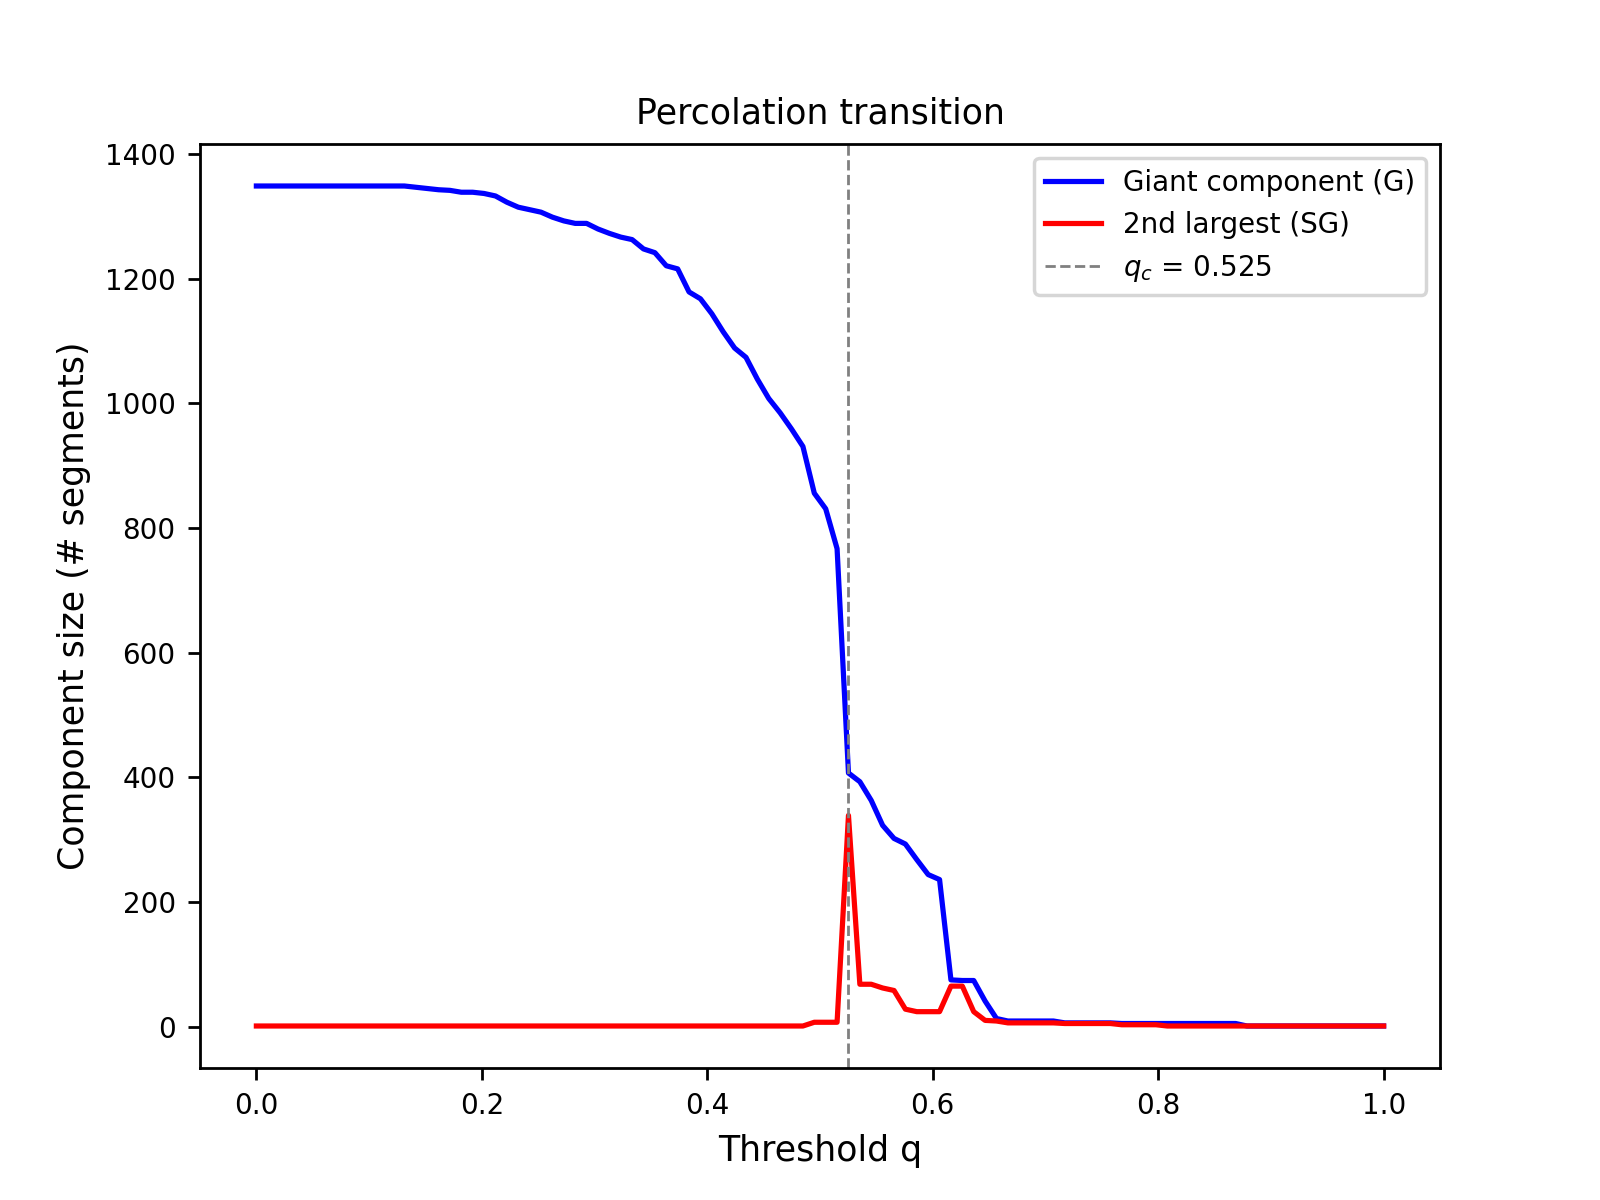
\includegraphics[width=0.72\textwidth]{percolation_transition.png}
  \caption{Percolation transition of the road network (session-and-time-averaged
    normalised speed).
    \textbf{Blue}: giant SCC size $G(q)$.
    \textbf{Red}: second-largest SCC size $S_G(q)$.
    The dashed vertical line marks $q_c = 0.52$, at which $S_G$ is maximised,
    indicating the onset of network-scale fragmentation.}
  \label{fig:percolation_transition}
\end{figure}

The percolation threshold $q_c = 0.52$ is retained for the main analysis because
it is data-driven, reproducible across sessions, and grounded in network topology.
The raw-speed threshold ($q = 2.0$\,m/s) is shown in parallel in
Section~\ref{sec:methods:congmaps} to illustrate the sensitivity to threshold
choice.

\subsubsection{Bottleneck Detection}
\label{sec:methods:bottlenecks}

As a by-product of the percolation sweep, segments whose normalised speed lies
in the marginal band $r_{ij} \in [q_c - \delta,\; q_c + \delta]$ with $\delta =
0.01$ are identified as \emph{bottlenecks}.  These links are barely functional at
$q_c$; their congestion would sever the bridges between functional sub-networks
and collapse the giant SCC.  Figure~\ref{fig:percolation_bottlenecks} shows their
spatial distribution on the simplified network.

\begin{figure}[H]
  \centering
  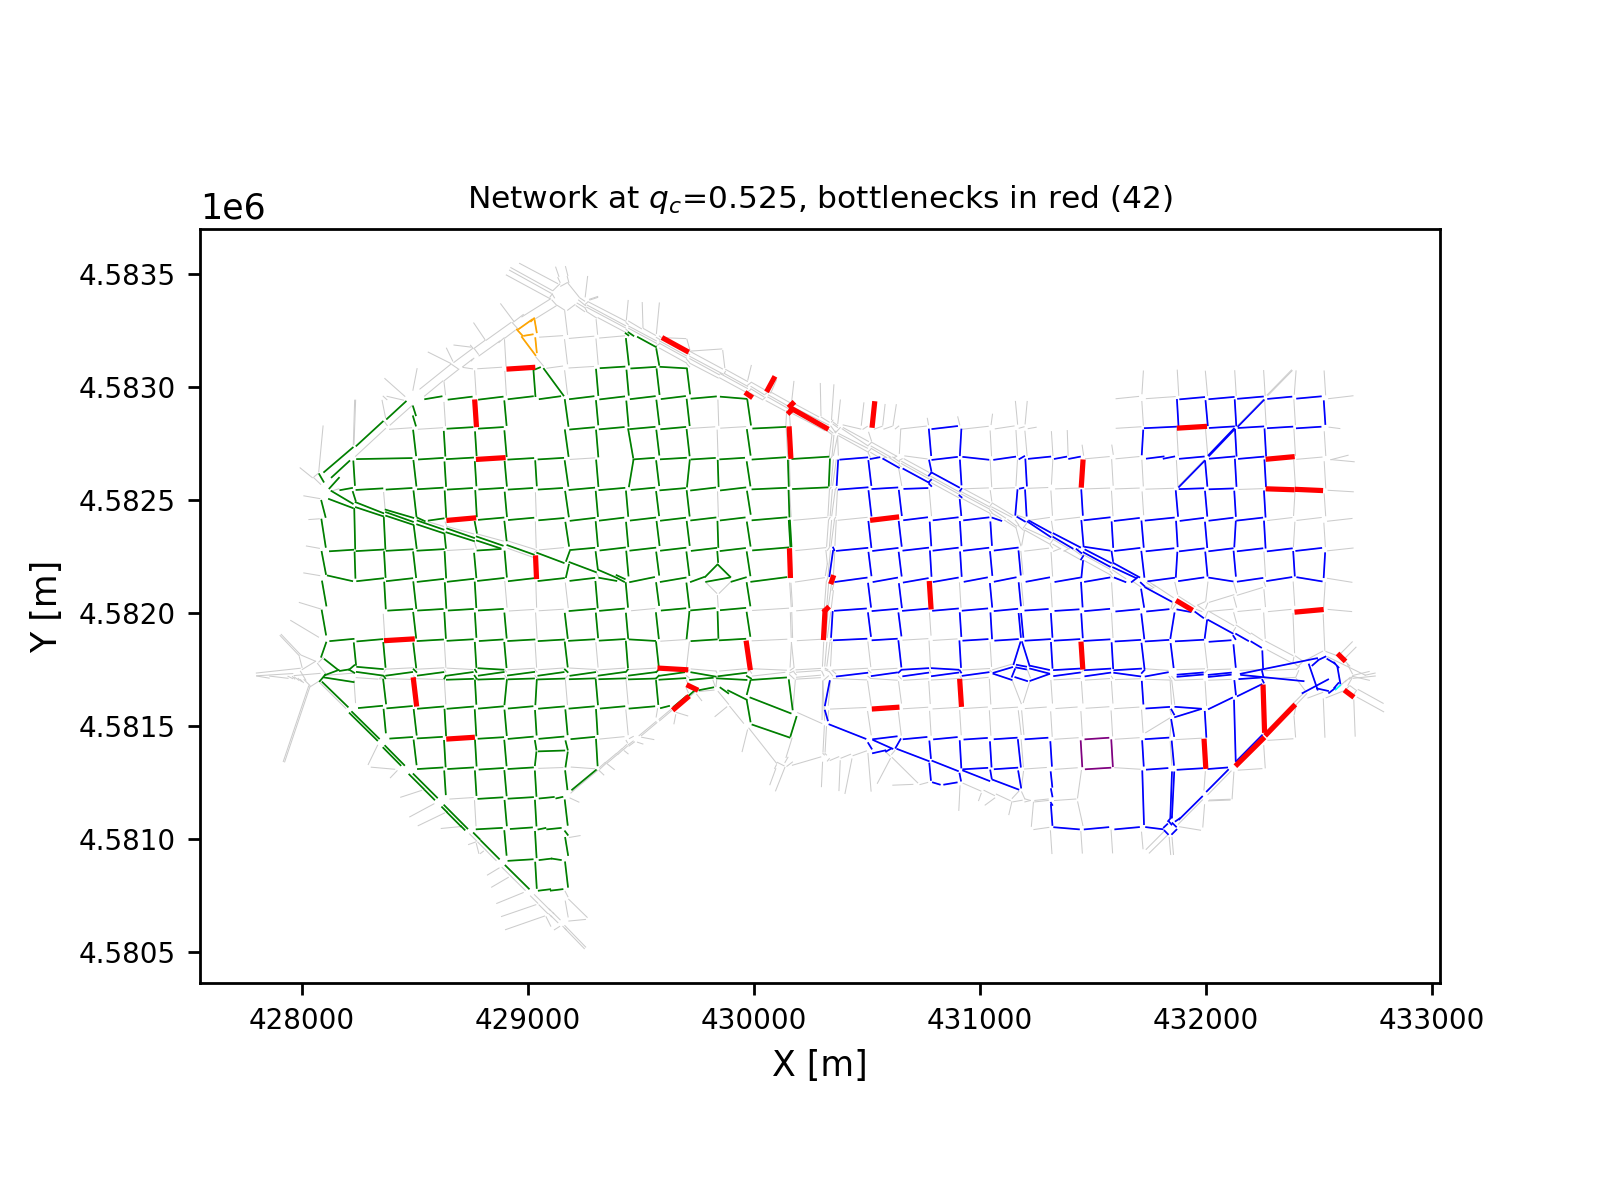
\includegraphics[width=0.88\textwidth]{percolation_bottlenecks.png}
  \caption{Network state at $q_c = 0.52$ (session-and-time-averaged, simplified
    graph).  Colours denote strongly connected components (green = giant SCC;
    blue, orange, purple, cyan = smaller SCCs).  Dark-red segments are congested
    ($r_{ij} < 0.52$); \textbf{thick red} segments are bottlenecks ($r_{ij} \in
    [0.51, 0.53]$); grey segments have insufficient data ($> 30\%$ missing
    observations).}
  \label{fig:percolation_bottlenecks}
\end{figure}

\subsubsection{BFS Connected-Component Analysis}
\label{sec:methods:bfs}

At each timestep $t$, the binary congestion map is constructed by labelling every
cell with $\bar{r}_c(t) < 0.52$ as congested.  A BFS with \textbf{8-connectivity}
(four cardinal directions plus four diagonals) then identifies every maximal
spatially contiguous set of congested cells as one component.  At the
$\approx 250\,\text{m}$ cell resolution, diagonal neighbours almost always share
road infrastructure; restricting to four-connectivity would artificially split
zones that are physically contiguous across a grid boundary.  Components are
ranked by descending size at each timestep (rank 1 = largest congested zone).  The
set of all functional cells ($\bar{r}_c \geq 0.52$) forms a single
\emph{uncongested background} cluster, giving the full $N(t) + 1$ partition used
for metric tracking.

\subsubsection{Results: Congestion Maps and Temporal Metrics}
\label{sec:methods:congmaps}

Figure~\ref{fig:graph_search_norm} shows the temporal evolution of the top-5
congested clusters under $q_c = 0.52$ (normalised speed, mean over all 101
sessions).  The three-row layout presents spatial maps at four selected timesteps
(top row), cluster sizes over time (middle), and median raw speed per cluster
over time (bottom).

\begin{figure}[H]
  \centering
  
\includegraphics[width=\textwidth]{graph_search/norm_q0.52/merged_graph_search_analysis.png}
  \caption{Approach~1 --- $q_c = 0.52$, normalised speed, mean over all sessions.
    \textbf{Top row}: BFS cluster maps at four representative timesteps.
    Congested clusters are ranked by size (rank~1 = red, rank~2 = blue,
    rank~3 = orange, etc.); functional cells are green; no-data cells are grey.
    \textbf{Middle}: number of grid cells in the top-5 congested clusters over
    time.
    \textbf{Bottom}: median raw speed (m/s) of segments within each cluster
    over time.  Vertical dashed lines indicate the timesteps shown in the top row.}
  \label{fig:graph_search_norm}
\end{figure}

Figure~\ref{fig:graph_search_raw} repeats the analysis with the manual raw-speed
threshold $q = 2.0$\,m/s.  This stricter criterion targets only near-standstill
traffic and establishes an upper bound on how severe congestion must be to
register as a connected zone under the manual threshold.

\begin{figure}[H]
  \centering
  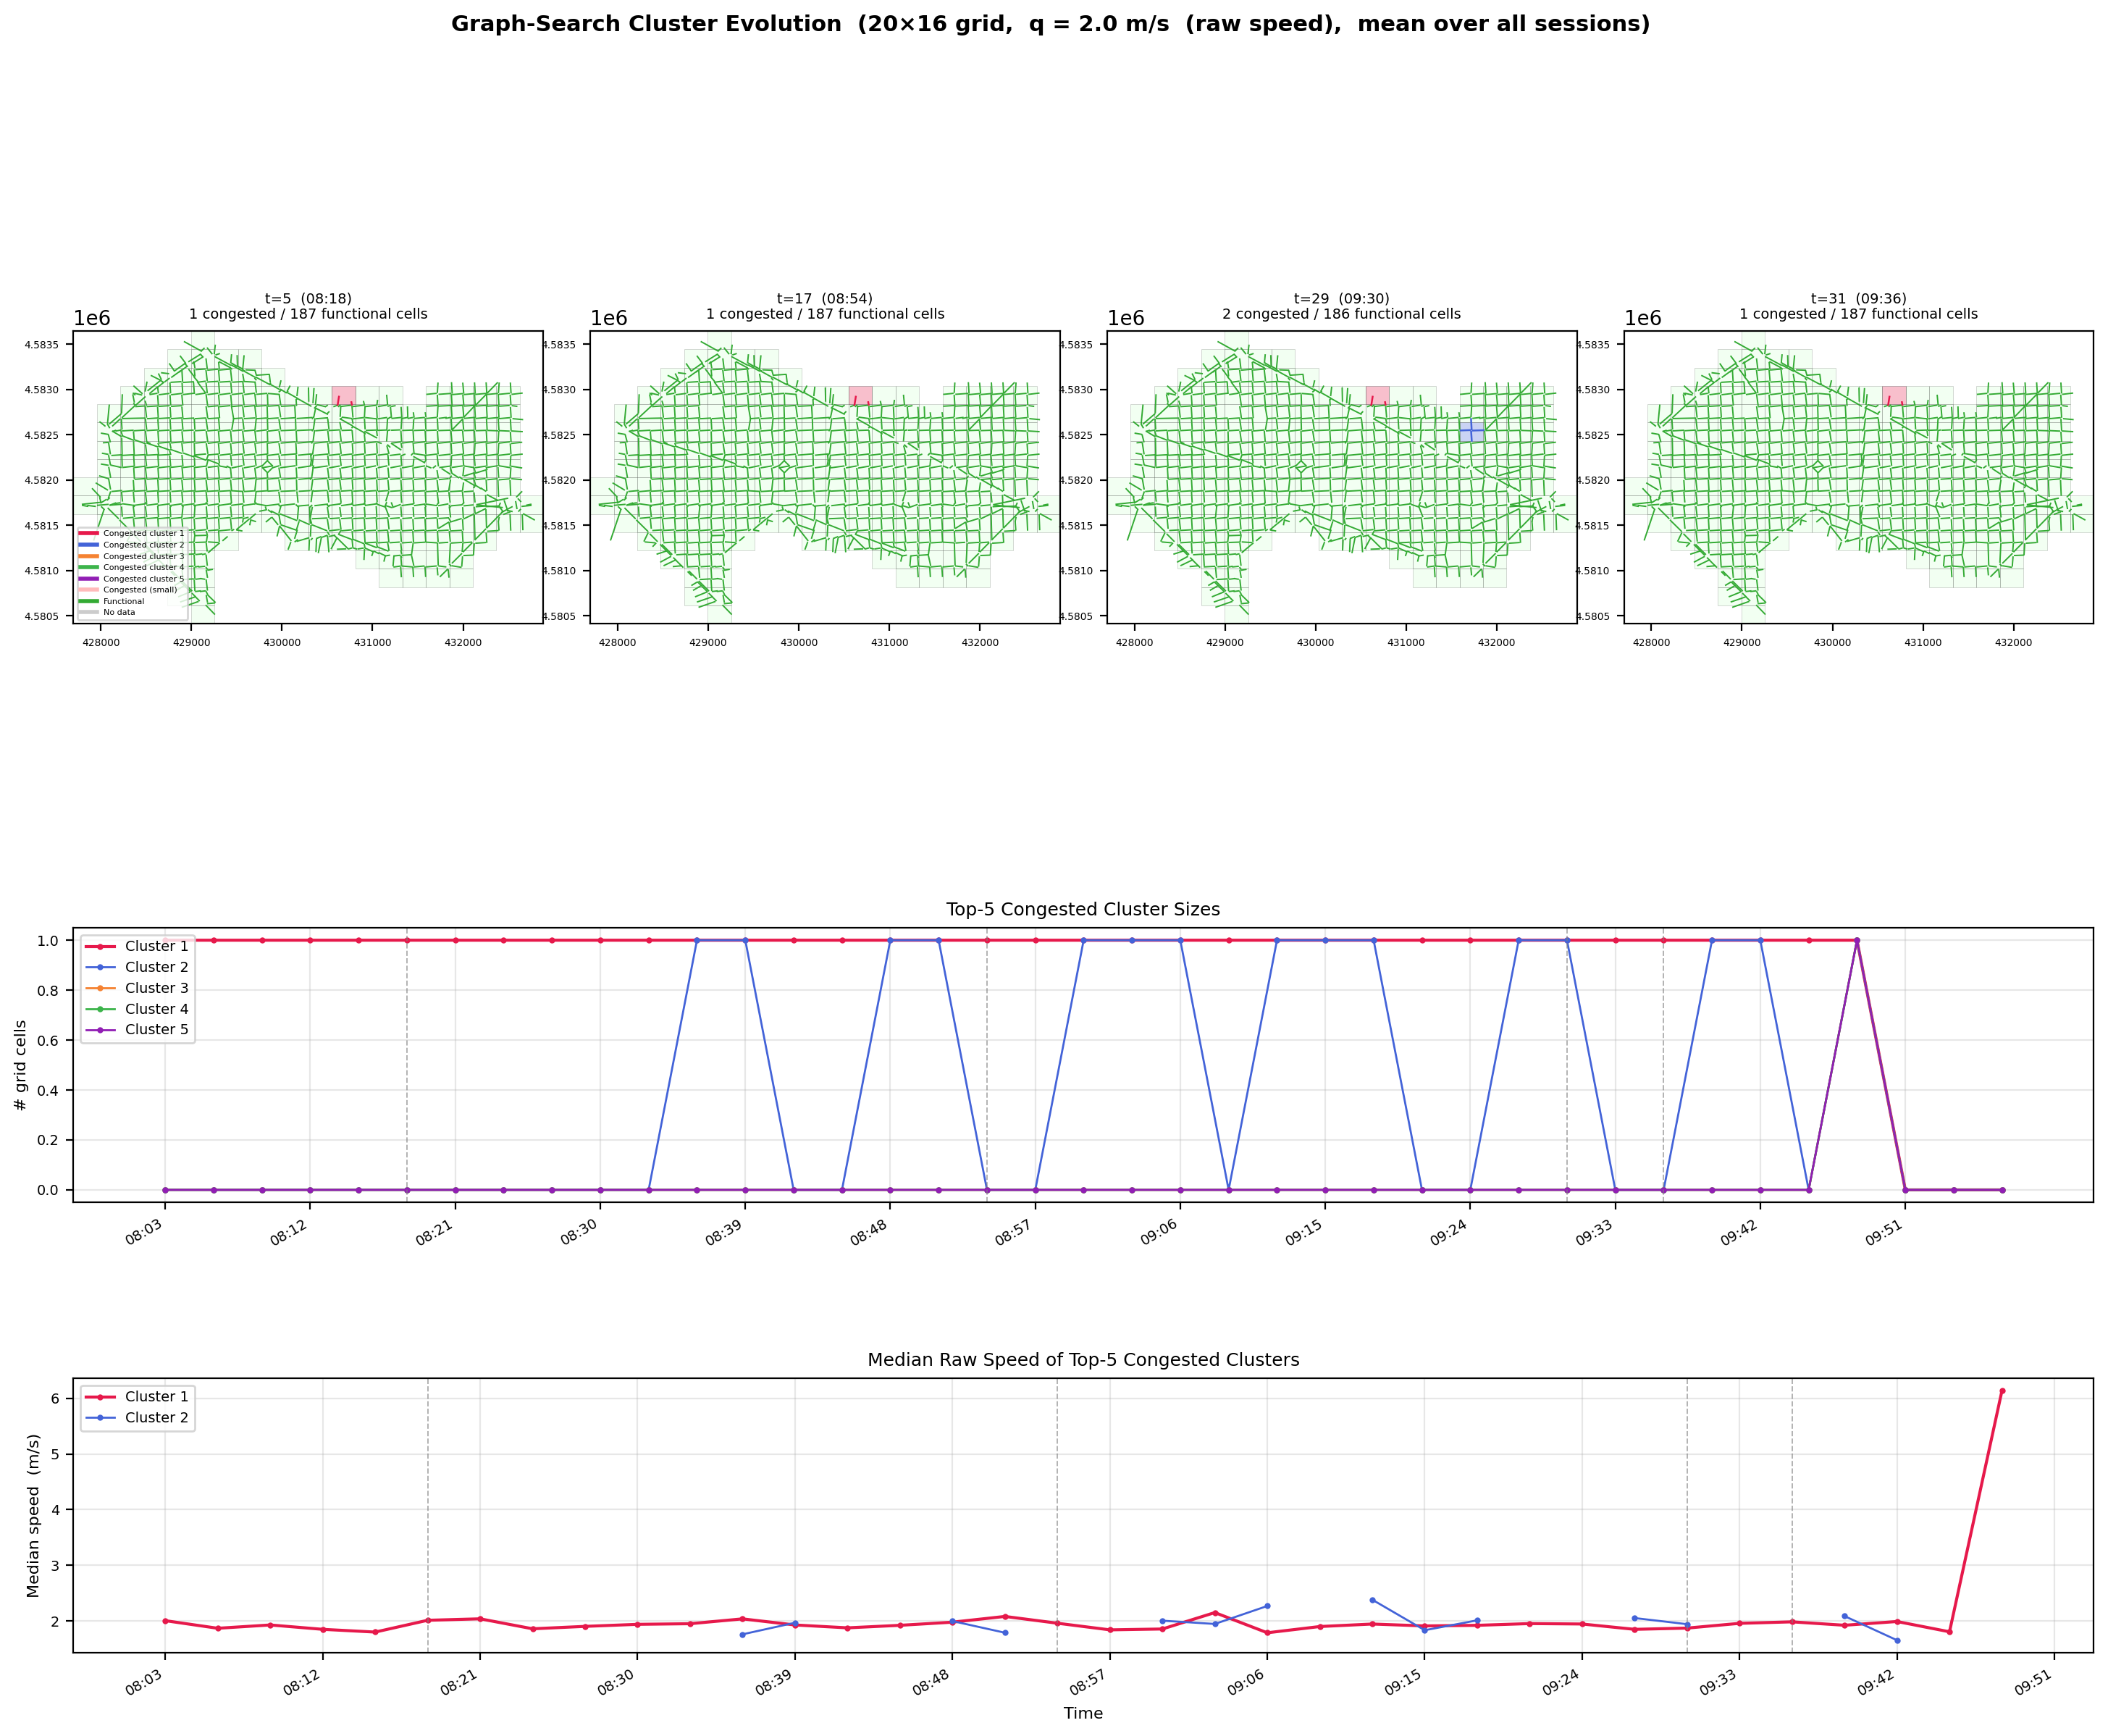
\includegraphics[width=\textwidth]{graph_search/raw_q2/merged_graph_search_analysis.png}
  \caption{Approach~1 --- $q = 2.0$\,m/s, raw speed.
    Layout identical to Figure~\ref{fig:graph_search_norm}.  Only
    near-standstill cells ($\bar{v}_c < 7.2$\,km/h) are labelled congested.}
  \label{fig:graph_search_raw}
\end{figure}

Table~\ref{tab:merge_metrics} reports the three evaluation metrics for
Approach~1 at the 15 representative timesteps under $q_c = 0.52$.  Clusters are
ranked by size at each timestep; the uncongested background is reported
separately.

\begin{table}[H]
  \centering
  \small
  \caption{Approach~1 metrics ($q_c = 0.52$, normalised speed, mean over all
    sessions).  $N$: number of congested BFS components.  $S_k$: size (grid
    cells) of rank-$k$ congested cluster.  $\tilde{v}_k$: median raw speed
    (m/s) of that cluster.  $\tilde{v}_{\mathrm{bg}}$: median speed of the
    uncongested background.}
  \label{tab:merge_metrics}
  \setlength{\tabcolsep}{5pt}
  \begin{tabular}{l c ccc ccc c}
    \toprule
    Time  & $N$ & $S_1$ & $S_2$ & $S_3$
          & $\tilde{v}_1$ & $\tilde{v}_2$ & $\tilde{v}_3$
          & $\tilde{v}_{\mathrm{bg}}$ \\
    \midrule
    08:03 & & & & & & & & \\
    08:12 & & & & & & & & \\
    08:18 & & & & & & & & \\
    08:24 & & & & & & & & \\
    08:30 & & & & & & & & \\
    08:42 & & & & & & & & \\
    08:54 & & & & & & & & \\
    09:00 & & & & & & & & \\
    09:06 & & & & & & & & \\
    09:12 & & & & & & & & \\
    09:18 & & & & & & & & \\
    09:30 & & & & & & & & \\
    09:42 & & & & & & & & \\
    09:51 & & & & & & & & \\
    09:57 & & & & & & & & \\
    \bottomrule
  \end{tabular}
\end{table}
% TODO: populate Table~\ref{tab:merge_metrics} from graph\_search/norm\_q0.52/ outputs.

% ──────────────────────────────────────────────────────────────────────────
\subsection{Approach~2 --- Grid K-means Clustering}
\label{sec:methods:clustering}

\subsubsection{Feature Construction and K-means Setup}
\label{sec:methods:gridkmeans}

Rather than applying a hard binary threshold, K-means partitions the grid cells
into $K$ clusters that jointly encode \emph{spatial position} and \emph{average
normalised speed}.  The feature vector for each non-empty cell $c$ is:
\begin{equation}
  \mathbf{x}_c \;=\; \mathrm{StandardScaler}\!\left(
    \bigl[\,\mathrm{cell}_x^{(c)},\;\mathrm{cell}_y^{(c)},\;\bar{r}_c\,\bigr]^\top
  \right),
  \label{eq:kmeans_features}
\end{equation}
where $\mathrm{cell}_x^{(c)}$ and $\mathrm{cell}_y^{(c)}$ are the integer grid
coordinates and $\bar{r}_c$ is the time-and-session-averaged normalised speed of
cell $c$.  Standard scaling normalises the three features to zero mean and unit
variance so that spatial extent and speed range contribute equally to the
Euclidean distance used by K-means.

K-means is fitted with k-means++ initialisation and 10 independent random
restarts; the lowest-inertia solution is retained.  Each resulting cluster is
labelled \emph{congested} if its mean normalised speed $\bar{r}_k < q_c = 0.52$,
and \emph{functional} otherwise.  Congested clusters are shown with a hatched fill
on maps.

The five cluster centroids in cell space are additionally mapped back to the
nearest road segment on the simplified network (the \emph{spawn points}), making
the partition interpretable at segment level and providing a spatially
well-distributed initialisation for further analyses.

\subsubsection{Cluster Count: $K = 5$ vs.\ $K = 9$}
\label{sec:methods:kselect}

Two values of $K$ are evaluated on the same grid and feature set:
\begin{itemize}
  \item \textbf{$K = 9$}: finer spatial granularity, better able to resolve
    distinct sub-congested zones within one geographic area.  Risk: a single
    physically coherent congested zone may be split into several clusters with
    similar speed profiles, reducing interpretability.
  \item \textbf{$K = 5$}: broader zones aligned with the network's macro-scale
    structure (roughly one cluster per urban district), yielding five clearly
    distinct, stable partitions.
\end{itemize}
The preferred $K$ is selected by comparing the three evaluation metrics and the
visual coherence of the partition; the result is reported in
Section~\ref{sec:methods:results_km}.

\subsubsection{Results}
\label{sec:methods:results_km}

Figure~\ref{fig:grid_kmeans_maps} shows the Grid K-means partition for $K = 5$
and $K = 9$ under $q_c = 0.52$.

\begin{figure}[H]
  \centering
  \begin{subfigure}[b]{0.48\textwidth}
    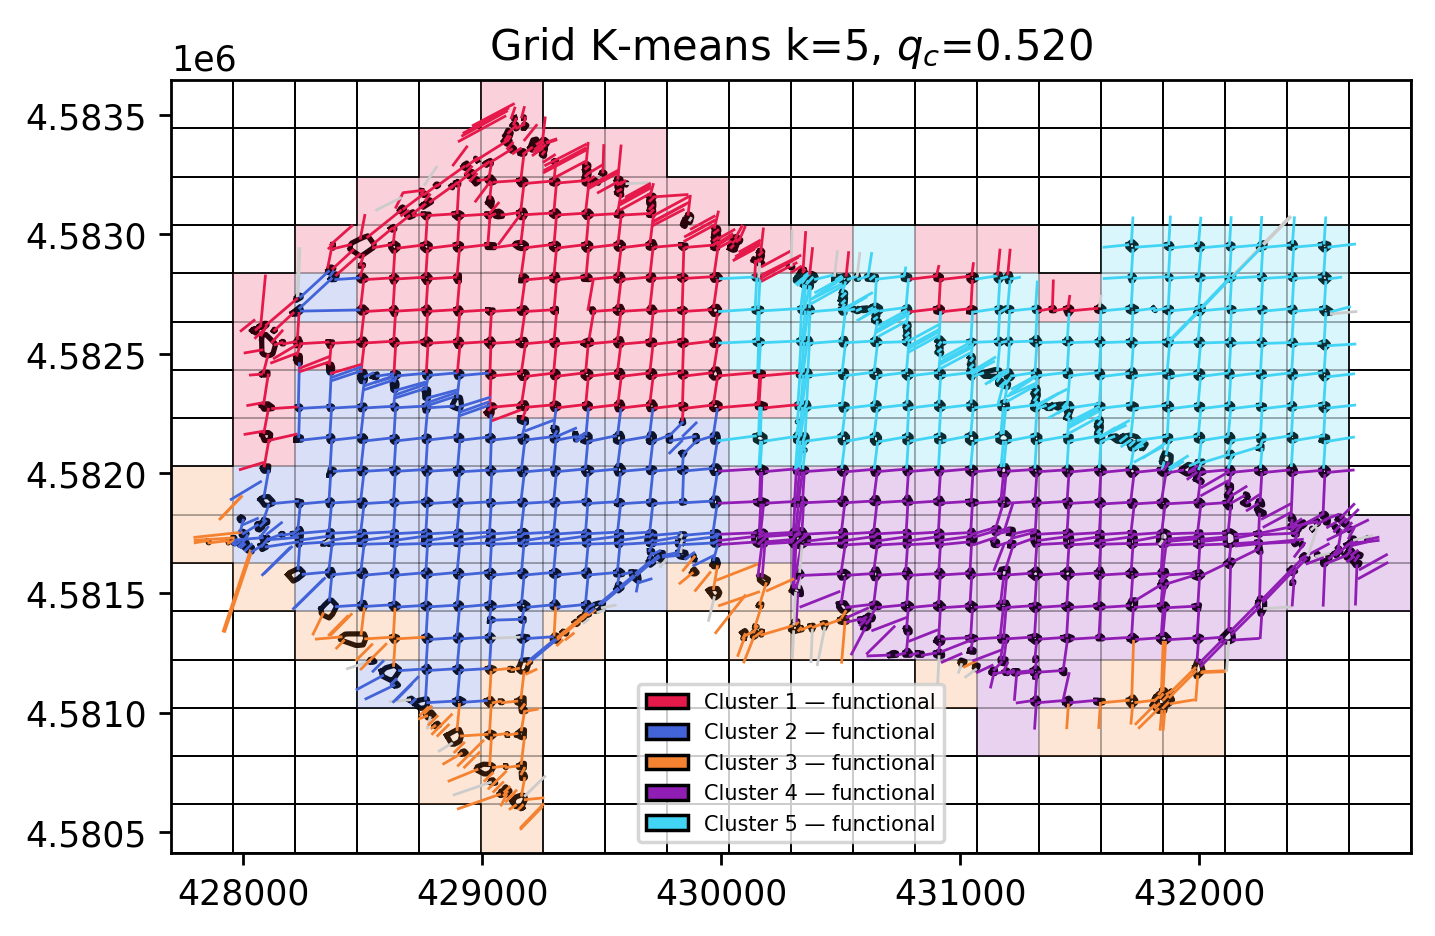
\includegraphics[width=\textwidth]{clustering/grid_clusters/grid_kmeans5_qc0.520.png}
    \caption{$K = 5$}
  \end{subfigure}
  \hfill
  \begin{subfigure}[b]{0.48\textwidth}
    % TODO: run grid\_clust\_kmeans(k=9, qc=0.52) to generate this figure.
    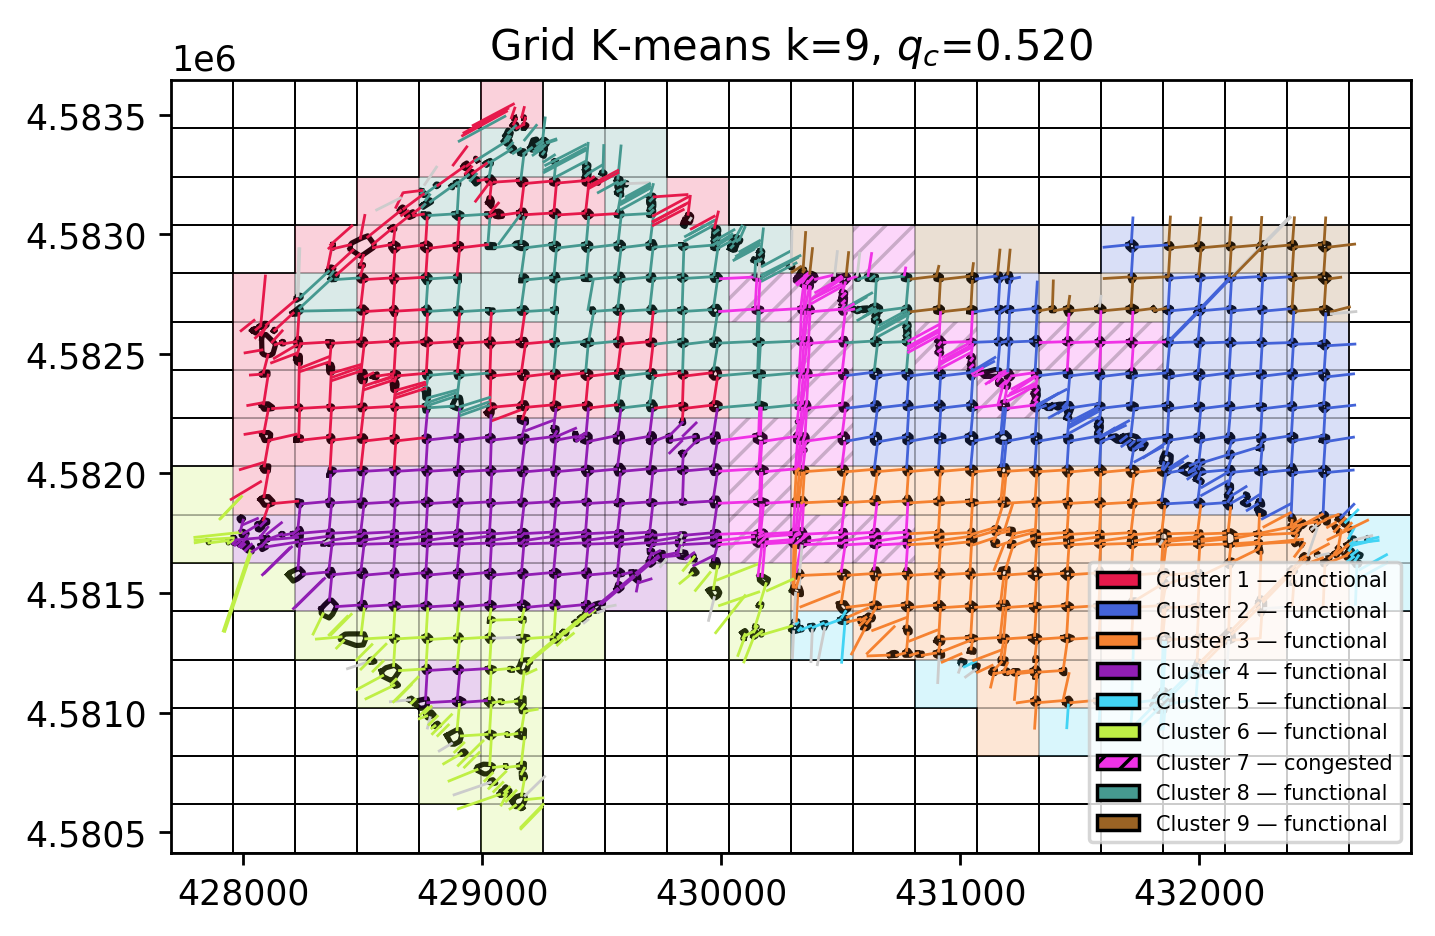
\includegraphics[width=\textwidth]{clustering/grid_clusters/grid_kmeans9_qc0.520.png}
    \caption{$K = 9$}
  \end{subfigure}
  \caption{Grid K-means partition at $q_c = 0.52$.  Each colour represents one
    cluster; hatching indicates clusters labelled congested (mean
    $\bar{r}_k < 0.52$).}
  \label{fig:grid_kmeans_maps}
\end{figure}

Figure~\ref{fig:grid_kmeans_speed} shows the median raw speed of each cluster
tracked over the 15 representative timesteps for the preferred $K$.

\begin{figure}[H]
  \centering
  % TODO: update path once preferred K is confirmed.
  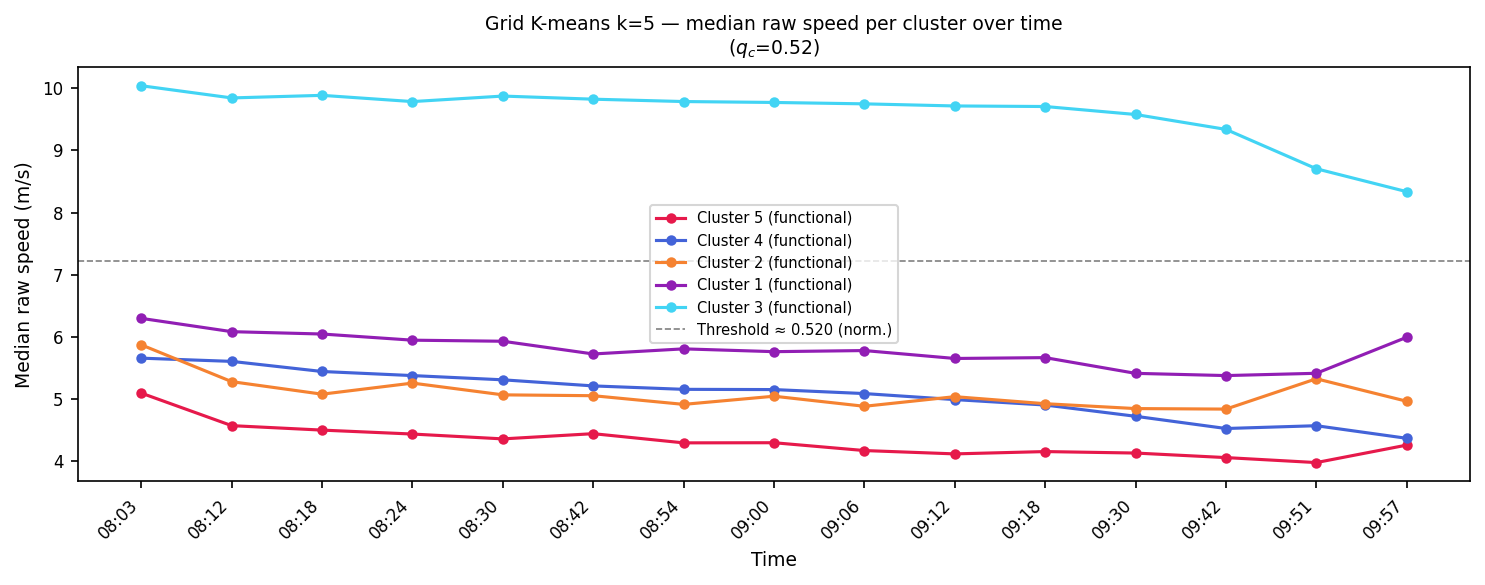
\includegraphics[width=\textwidth]{clustering/grid_clusters/grid_kmeans5_qc0.520_median.png}
  \caption{Grid K-means (preferred $K$): median raw speed (m/s) per cluster over
    the analysis window.  Congested clusters (hatched in
    Figure~\ref{fig:grid_kmeans_maps}) show persistently lower speeds throughout
    the peak period.}
  \label{fig:grid_kmeans_speed}
\end{figure}

Table~\ref{tab:km_metrics} reports the three evaluation metrics for Approach~2
at the 15 representative timesteps using the preferred $K$.  Clusters are ordered
by mean speed (ascending), so cluster~1 is the most congested zone.

\begin{table}[H]
  \centering
  \small
  \caption{Approach~2 metrics (Grid K-means, preferred $K$, $q_c = 0.52$).
    $N_c$: number of clusters labelled congested.  $S_k$: size (grid cells) and
    $\tilde{v}_k$: median raw speed (m/s) of cluster $k$, ordered by ascending
    mean speed.}
  \label{tab:km_metrics}
  \setlength{\tabcolsep}{4pt}
  \begin{tabular}{l c ccccc ccccc}
    \toprule
    Time & $N_c$ & $S_1$ & $S_2$ & $S_3$ & $S_4$ & $S_5$
         & $\tilde{v}_1$ & $\tilde{v}_2$ & $\tilde{v}_3$ & $\tilde{v}_4$
         & $\tilde{v}_5$ \\
    \midrule
    08:03 & & & & & & & & & & & \\
    08:12 & & & & & & & & & & & \\
    08:18 & & & & & & & & & & & \\
    08:24 & & & & & & & & & & & \\
    08:30 & & & & & & & & & & & \\
    08:42 & & & & & & & & & & & \\
    08:54 & & & & & & & & & & & \\
    09:00 & & & & & & & & & & & \\
    09:06 & & & & & & & & & & & \\
    09:12 & & & & & & & & & & & \\
    09:18 & & & & & & & & & & & \\
    09:30 & & & & & & & & & & & \\
    09:42 & & & & & & & & & & & \\
    09:51 & & & & & & & & & & & \\
    09:57 & & & & & & & & & & & \\
    \bottomrule
  \end{tabular}
\end{table}
% TODO: populate Table~\ref{tab:km_metrics} once preferred K is confirmed.

% ──────────────────────────────────────────────────────────────────────────
\subsection{Comparative Analysis}
\label{sec:methods:comparison}

Table~\ref{tab:comparison} places the key metrics of both approaches side by
side at seven representative timesteps spanning the full rush-hour window.  The
two methods are compared on the number of congested clusters they identify, the
size of the largest congested zone, and the median speed within it.  Qualitative
differences in spatial layout are discussed with reference to
Figures~\ref{fig:graph_search_norm} and~\ref{fig:grid_kmeans_maps}.

\begin{table}[H]
  \centering
  \small
  \caption{Side-by-side comparison of Approach~1 (BFS, $q_c = 0.52$) and
    Approach~2 (Grid K-means, preferred $K$, $q_c = 0.52$) at seven
    representative timesteps.  $N$: number of congested clusters.  $S_1$: size
    (grid cells) of the largest congested cluster.  $\tilde{v}_1$: its median
    raw speed (m/s).}
  \label{tab:comparison}
  \setlength{\tabcolsep}{5pt}
  \begin{tabular}{l rr rr rr}
    \toprule
    & \multicolumn{2}{c}{$N$ congested clusters}
    & \multicolumn{2}{c}{$S_1$ (grid cells)}
    & \multicolumn{2}{c}{$\tilde{v}_1$ (m/s)} \\
    \cmidrule(lr){2-3}\cmidrule(lr){4-5}\cmidrule(lr){6-7}
    Time & BFS & K-means & BFS & K-means & BFS & K-means \\
    \midrule
    08:03 & & & & & & \\
    08:18 & & & & & & \\
    08:42 & & & & & & \\
    09:00 & & & & & & \\
    09:18 & & & & & & \\
    09:42 & & & & & & \\
    09:57 & & & & & & \\
    \bottomrule
  \end{tabular}
\end{table}
% TODO: populate Table~\ref{tab:comparison} once both result sets are finalised.

% ══════════════════════════════════════════════════════════════════════════
\section{Evaluation}
\label{sec:eval}

\subsection{Evaluation framework}
\label{sec:eval:framework}
% What we are measuring: spatial coherence, temporal stability, separability,
% interpretability.
% TODO

\subsection{Metrics}
\label{sec:eval:metrics}

\subsubsection{Internal cluster-quality metrics}
% Silhouette, Davies--Bouldin, inertia.
% TODO

\subsubsection{Stability metrics}
% Cross-session stability, sensitivity to $k$, sensitivity to weights.
% TODO

\subsubsection{Spatial-coherence metrics}
% Compactness, fragmentation, neighbour agreement.
% TODO

\subsubsection{Congestion-recovery metrics}
% Agreement with threshold/percolation labels.
% TODO

\subsection{Choosing the number of clusters}
\label{sec:eval:k}
% evaluate\_k figures: $k=4..8$, conclusion.
% TODO

\subsection{Results — Merge methods}
\label{sec:eval:merge}

\subsubsection{Threshold and grid aggregation}
% TODO

\subsubsection{Percolation transition and bottlenecks}
% TODO

\subsection{Results — Clustering}
\label{sec:eval:clustering}

\subsubsection{K-means: speed / distance / time / geometric features}
% TODO

\subsubsection{K-means with bottleneck weighting}
% TODO

\subsubsection{K-means stability across sessions}
% TODO

\subsubsection{Ward vs.\ K-means}
% TODO

\subsection{Comparison of the two approaches}
\label{sec:eval:compare}
% Where they agree, where they disagree, complementarity.
% TODO

\subsection{Limitations}
\label{sec:eval:limits}
% NaN coverage, session imbalance, parameter sensitivity.
% TODO

% ══════════════════════════════════════════════════════════════════════════
\section{Conclusion}
\label{sec:conclusion}

\subsection{Summary of findings}
% TODO

\subsection{Future work}
% TODO

% ══════════════════════════════════════════════════════════════════════════
\appendix

\section{Implementation overview}
\label{app:impl}
% Module map: config, processing.speed, network.{draw,simplify},
% clustering.{features,kmeans,ward}, percolation.{core,maps}, gif, utils.
% TODO

\section{Parameter reference}
\label{app:params}
% TODO

\bibliographystyle{plain}
\bibliography{references}

\end{document}
